\documentclass[UKenglish]{ifimaster}
\usepackage[utf8]{inputenc}
\usepackage[T1]{fontenc,url}
\urlstyle{sf}
\usepackage{babel,textcomp,csquotes,duomasterforside,varioref,graphicx}
\usepackage[backend=biber,style=numeric-comp]{biblatex}
%\usepackage{color}   %May be necessary if you want to color links
%\usepackage[hidelinks]{hyperref}
\usepackage{hyperref}
\usepackage{listings}
\usepackage{graphicx}
\usepackage{etoolbox}
\usepackage[newfloat]{minted}
\usepackage{caption}
\hypersetup{
   colorlinks=false, %set true if you want colored links
   linktoc=all,     %set to all if you want both sections and subsections linked
   %linkcolor=black,  %choose some color if you want links to stand out
}

\newenvironment{code}{\captionsetup{type=listing}}{}
\SetupFloatingEnvironment{listing}{name=Source Code}
\newcommand{\problemStatement}{How can Machine learning be used in different ways to predict bipolar disorder?}

\title{\problemStatement}
\subtitle{
% Subtitle %
}

\author{Joakim I. Frogner}
 
\bibliography{bibliography}

\begin{document}
\duoforside[dept={Department of Informatics},
program={Programming and Networks},
long]

\frontmatter{}
\chapter*{Abstract}

\tableofcontents{} 
\listoffigures{}
\listoftables{}

\chapter*{Preface}

\mainmatter{}
\part{Introduction}

\chapter{Introduction}
%%%%%% INTRODUCTION %%%%%%

\section{Motivation}
Ways to use the results of this study? 

\section{Thesis overview}
[Fill in later]



\chapter{Background}

The fields of studies for this thesis are both mental health and ML, and this chapter contains background information and previous research within both of them. We start with mental health, where we describe mental issues, depression, and bipolar disorder. Then we dive into the topic of ML, where we provide a technical introduction.

\section{Mental health}
Mental health problems are not known very well by the public. Jorm et al. performed research \cite{jorm1997mental} where they displayed vignettes of one patient suffering from major depression and one from schizophrenia to the people of the Australian public. Of the participants, only 39\% correctly guessed depression, and 27\% correctly guessed schizophrenia. Another study has shown that schizophrenia is often confused with multiple personalities \cite{angermeyer1999social}. Such poor public knowledge about mental health problems can be problematic, as people may have a condition without knowing anything about it. When this is the case, professional help use more time to establish their diagnosis. 

\subsection{Depression Rating: MADRS}
Montgomery-Åsberg Depression Rating Scale, or MADRS for short, is a rating system for telling how depressed a patient is. Stuart A. Montgomery and Marie Åsberg designed it in 1979, and it is more sensitive to changes than the Hamilton Rating Scale for Depression (HRS) for patients that go through antidepressant medication. The process for calculating a MADRS rating contains ten statements about the patient's behavior, where the topics are: apparent sadness, reported sadness, inner tension, reduced sleep, reduced appetite, concentration difficulties, lassitude, inability to feel, pessimistic thoughts, suicidal thoughts \cite{madrs_paper}.


The person doing the rating answers each question with a number between 0 and 6, where the higher the number, the more relevant the statement is for the patient. The numbers added together gives us the total MADRS score, which we split into four categories: normal/not depressed: 0-6, mild depression: 7-19, moderate depression: 20-34 and severe depression: 34-60 \cite{sunnybrook_stroke_study}. 

\subsection{Bipolar Disorder}

Bipolar disorder is the syndrome with extreme mood swings, referred to as \emph{mania} and \emph{depression} \cite{bipolar_disorder}. One day the person can feel amazing, and everything is fine, 
but the next day they feel like they do not belong anywhere in this universe. In general, one should be concerned about mood swings. 
It is, however, the extreme cases where the mind turns 180 degrees from day to day that is the main symptom of bipolar disorder. 
There is not a specific type of people that get this; they can be of any age and any gender, but most people that suffer from it find out 
(by having an experience or episode) around age 25 \cite{bipolar_statistics}. 

When talking about bipolar disorder, we often separate between the states \emph{normal}, \emph{mania} and \emph{depression}. 
The last two are the states we usually talk about since a normal state is not that interesting. These two states are very different, 
but they have some similarities, for example sleeping problems. When a bipolar person is in a manic state, he/she may feel so excited and powerful that they do things that they would never have intended doing, like spending much money on items they do 
not need \cite{bipolar_disorder}.

A bipolar patient is in a depressive state when he or she is in a bad mood swing. They can stop doing everything they usually like to do, 
and lie down in bed all day with no motivation to do anything useful. They may feel useless and that they do not belong here, 
or being guilty of something they may or may not have done. In some cases, depression may even end up with suicidality, 
where the person either spends much time thinking of death, or attempt suicide.

The frequency of these symptoms can vary. One year they can have these mood swings every day for several weeks at the time, and the next they get them less frequent, 
like once every month. We also separate between bipolar disorder type I and II, with the main difference being that the manic episodes are way 
more aggressive in type I \cite{bipolar_types}. Statistics say that bipolarity is genetically inheritable, with 23\% chance of getting a child with bipolar 
disorder if one parent is bipolar, and 66\% if both parents are \cite{bipolar_statistics}. 

\section{Machine learning}
ML is the field of computer science where we throw data into an algorithm and expect it to give answers to whatever the goal is, 
with as little work as possible. The process of performing ML was not as simple in the early days of the technology, 
but nowadays it is a lot easier with all the different frameworks and tools available.

ML is a tremendous and almost magical technology, but knowing how one should use it can be difficult without the experience. 
The amount of data needed to make an algorithm learn something makes it difficult to get started, and to be efficient when training the model on a large dataset, 
decent hardware is required. One can get away with using a CPU if they want to test ML on a small dataset, but if the goal is to build something useful, 
too much time is saved using a GPU. 

The reason why GPUs are so much better than CPUs on this specific task is that the design choices of a CPU are for flexibility and general computing workloads. 
The GPU, on the other hand, is designed to do simple arithmetic instructions over and over again (easy to parallelize). These design choices make GPUs a lot more 
efficient for ML, and especially for deep neural networks \cite{cpu_vs_gpu_ml}. Alternatively, if investing in a GPU is not the preferred choice, 
there are many cloud services available to us today where we can pay a small sum in order to use a system that is a better fit for the task.

Now how do we make a machine learn? Well, there are many different approaches to this, which we will discuss in the next sections, but let us say we want to 
use a neural network for achieving some goal. Then our next step should be to choose a framework. We can, of course, do everything from scratch, but why 
reinvent the wheel when there are so many good frameworks and tools already out there? 

Python is a programming language perfect for ML in our opinion. The language looks a lot like pseudo-code, and this is perfect because we do not 
want to spend time on syntax rules in another language. A popular framework called \textbf{TensorFlow} is available to use in Python, and developers from Google have built it. 

TensorFlow allows the programmer to build models quickly, and also execute the training and testing. TensorFlow can be used directly, but using \textbf{Keras} as an abstraction layer above it is a popular choice, which we did when implementing the neural networks for our objectives. On their documentation website \cite{keras_docs}, they describe their framework as \blockquote{A high-level neural networks API, written in Python and capable of running on top of TensorFlow, CNTK or Teano}.

Following their \textit{30 seconds to Keras} guide \cite{keras_docs}, you can create a \textit{sequential} model with \textit{dense}
layers, configure its learning process (compile), then fit, train, evaluate and predict with just a few lines of code \ref{code:keras-guide}.

\begin{code}
  \begin{minted}[linenos]{python}
      from keras.models import Sequential
      from keras.layers import Dense
  
      model = Sequential()
  
      model.add(Dense(units=64, activation='relu', input_dim=100))
      model.add(Dense(units=10, activation='softmax'))
  
      model.compile(loss='categorical_crossentropy',
                optimizer='sgd',
                metrics=['accuracy'])
      
      model.fit(x_train, y_train, epochs=5, batch_size=32)
      loss_and_metrics = model.evaluate(x_test, y_test, batch_size=128)
      classes = model.predict(x_test, batch_size=128)
  \end{minted}

  \caption{\textit{Simple introduction to Keras, where we create a Sequential model with two Dense layers, compile it with with the loss function Categorical Crossentropy and the optimizer SGD}}
  \label{code:keras-guide}
\end{code}


One thing that Keras does not make any easier is structuring the dataset so that the model can fit it. There is a high chance that we have to write some 
code ourselves to do this. Numpy is a package for Python built for math operations where everything happens optimally (Python by itself adds overhead to everything). 
All Python based ML algorithms assume that the input data is Numpy arrays, so experience with Numpy can be advantageous when structuring the dataset.

\section{Machine learning strategies}
Picking the right ML model can be quite tricky, especially for an inexperienced programmer. There are a couple of different \textit{strategies} one can choose 
from when deciding on an ML model. These are called \textit{supervised and unsupervised learning}, and we need to think about how the dataset is structured, 
and what we want to achieve to find out which one to use. The following sections will be a description of the strategies, to make the decision easier.

\subsection{Supervised learning}
Supervised learning is the ML strategy where we provide both input and correct output data to the algorithm \cite{supervised_learning}. 
We may use supervised learning if the goal is to train a model to classify letters in the alphabet, or something else where we have a dataset with both input 
and output data (for the alphabet, images of letters are input data, and the actual letters are the output data). If we train this alphabet detection model, 
we will be able to input an image (not seen before by the algorithm) of a letter, and the model will classify it to the letter it most likely correct. 
This kind of supervised learning is called \textit{Classification} and is the problem of assigning new observations to the class they most likely belong, 
based on a classification model built from labeled training data \cite{supervised_learning}.

Another kind of supervised learning is called \textit{Regression} and is all about predicting (or estimating) a value. A classic example of regression 
learning is predicting income, using \textit{features} like home, location, job title, the field of study,  years of education and years of experience. 
We call these features \textit{categorical} (first three) and \textit{numerical} (last two) \cite{supervised_learning}. 

\subsection{Unsupervised learning}
Another strategy is unsupervised learning. We want to use this if we have a dataset without the same meaning as in a dataset for supervised learning. 
The items may not have a fixed answer, like the letters in the alphabet are. It is useful when we have unlabeled data and want to for example group data 
together in what we call a \textit{cluster}. Unsupervised learning may not be as common as supervised learning, but it can be quite 
beneficial in some cases; for example when grouping addresses together in neighborhoods if we have an unsorted list of addresses as the dataset. Patterns are given to the algorithm, but no \textit{answers} are provided \cite{unsupervised_learning}. 

\subsection{Semi-supervised learning}
We may not always want to use one of the strategies above. Looking at the dataset, maybe we want something in between like a combination of labeled and unlabeled data. Semi-supervised learning comes in handy when this is the case. For example, if we have many data samples to label in our dataset, it can be too much work. We will not go deep into details about how this works, but it is essential to mention it because of its usefulness. The goal of semi-supervised learning is to understand how combining labeled, and unlabeled data may change the learning behavior, and design algorithms that take advantage of such a combination \cite{semisupervised_learning}.

\section{Machine learning approaches}
When we know whether we want to use supervised learning, unsupervised learning or something in between, we need to select an approach. We use the term approach because we use these regardless of the strategy, as most approaches work in both supervised and unsupervised learning. There are a lot of different approaches available, and we will describe some of them.

\subsection{Decision tree learning}
\begin{table}[h]
    \centering
    \begin{tabular}{| l | l | l | l | l | l |}
    \hline
    \textbf{Day} & \textbf{Temperature} & \textbf{Outlook}   & \textbf{Humidity}  & \textbf{Wind}     & \textbf{Run} \\ \hline
            1    & 15 C                 & Sun                & Low                & Strong            & Yes \\
            2    & 6 C                  & Rain               & High               & Weak              & No  \\
            3    & 15 C                 & Rain               & Medium             & Strong            & Yes \\
            4    & 6 C                  & Overcast           & High               & Medium            & Yes \\
            5    & 15 C                 & Sun                & Low                & Weak              & No  \\
            6    & 12 C                 & Overcast           & Medium             & Weak              & No  \\
            7    & 12 C                 & Sun                & Medium             & Medium            & Yes \\
    \hline
    \end{tabular}
    \caption{Example training data set: days a person went out for a run}
    \label{table:days_running}
\end{table}

In computer science, trees are data structures commonly used to describe something that \textit{branches out} based on different input. For example, 
a tree can be a representation of how the frequency of letters in the alphabet are distributed in a text file so that the text file can be compressed optimally. 
We will not go into details about how this works, but our point is that tree-structures are very common in most fields of computer science. 

In ML, we can apply the tree-structures as \textit{decision tree learning}. Decision trees are trees that classify instances by sorting them based on feature values, and each \textit{node} represents a feature. Each branch represent a value that the node can assume \cite{supervised_learning}.
In this approach, we set up all the different outcomes (with the training data set) of a specific question in a tree. Let us say we want to predict whether or not a person will run outside on a specific day. 
Then it makes sense that the training set contains weather information. The different data in the training set is called attributes, and correctly picking 
these is essential for the quality of the prediction.

Table \ref{table:days_running} contains data about whether a person went outside for a run or not for a week (just an example, not real data). 
Here the first 4 (excluding "Day") columns (Temperature, Outlook, Humidity, and Wind) is the "predictors" and the last column (Run) is the target. 
To use this table in decision tree learning, we need to view it as a tree, with one of the predictors as the root node and the targets as leaf nodes. 

How we choose the tree structure is critical to the performance of the ML, and we need to use a good tree building algorithm. 
The most common algorithm to use in this situation is the \textit{ID3} algorithm made by J. R. Quinlan. It is a top-down, greedy search through the space 
of possible branches with no backtracking \cite{decision_tree}. The way this happens is by calculating \textit{Entropy} and \textit{Information Gain}. 
The idea is to recursively choose the predictor that has the highest information gain and generate a tree structure. With an optimal tree, 
we can create decision rules by merely following the tree with new data.

\subsubsection{Random Forest}
One known problem with decision tree models is that they often include much \textit{variance}. Variance in an algorithm means that it is sensitive to small 
changes in the training set. One method to reduce the variance is to use Random Forest. 

Random forests are a combination of tree predictors such that each tree depends on the values of a
random vector sampled independently and with the same distribution for all trees in the forest \cite{random_forest}. 
It is a supervised ML strategy and can be useful for both classification and regression learning.

For example, if we want to get movie recommendations using ML, using one decision tree will most likely be insufficient. 
Just think what happens when we ask a friend for movies to watch. What that friend recommends is purely based on movies we like ourselves and what the friend likes. 
We might be lucky and find our next favorite movie, but most likely, asking multiple people for recommendations is going to yield better results. 
The same goes for ML, and decision trees will most likely give a better answer if we combine them in a Random Forest.

\subsection{Deep Neural Networks}

\begin{figure}[!ht]
    \begin{center}
        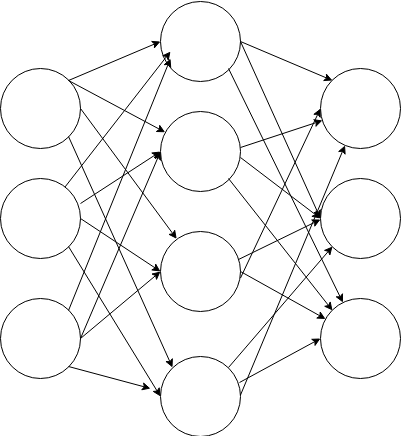
\includegraphics[height=10cm]{neural_net.png}
        \caption{Neural network visualization. The inputs on the left side are passed into the neurons in the hidden layer in the middle, which passes the values to the output layer.}
        \label{figure:neural_net}
    \end{center}
\end{figure}

The general idea of ML with neural networks is to make the computer think like a human, inspired by the way biological neural networks in the human brain process information \cite{deep_learning}. There are a lot of different neural network architectures, but all of them share the same underlying layer-based architecture, where data get passed between layers where computation happens. The first layer is the input layer, which passes the data to the next layer, which is the hidden layers. The number of hidden layers is entirely up to the model and the programmer, and this is where the intermediate processing/computation is done before the data get passed to the output layer where we perform an activation function to define the output \cite{deep_learning}.

Figure \ref{figure:neural_net} is a visual representation of a neural network with the input layer on the left, one hidden layer in the middle and the output layer on the right-hand side. For each layer, we have fully connected nodes, which means that each node has a connection to all nodes in the next layer.

If we have multiple hidden layers in a neural network, we call it a \textit{deep} neural network (DNN). DNNs can be useful for anything, and only the programmer's creativity sets the limit. Two common ways to use DNNs are \textit{Recurrent Neural Networks (RNNs)} and \textit{Convolutional Neural Networks (CNNs)}. These two have their use cases, which we will describe further.

\subsubsection{Recurrent Neural Network (RNN)}
RNNs are useful for predicting something based on a sequence of data, like for example predicting words in a sentence, which can be especially useful for typing on the phone. Also making predictions based on historical data, speech and language, are tasks an RNN can do effectively \cite{deep_learning}.

One downside to RNNs used on large sequences of data is that the prediction will most likely be off if a word written at the beginning of a long text is a dependency for a prediction four chapters later, for example, the home location of the main character. The workaround for this is something called \textit{Long Short-Term Memory Recurrent Neural Network (LSTM RNN)}, and is the idea of having additional logic to avoid the prediction model forgetting essential facts \cite{deep_learning}.

\subsubsection{Convolutional Neural Network (CNN)}
A CNN can be used for identifying patterns in data, which then is the underlying calculations for either prediction or classification. They are designed to process data in different array shapes \cite{deep_learning}. A common use case for CNNs is image recognition. In image recognition, we train our models to be good at identifying objects in images, for example, the difference between cats and dogs. Then we can input a completely different image to the model, and it will output whether the image is of a cat or a dog. 

This type of CNN is two-dimensional because an input image is a two-dimensional array of pixels, so the network also needs to have two dimensions in the convolutional layers. Another way of constructing a CNN is one-dimensionally, which can be useful for \textit{one-dimensional} data, for example, sensor data from gyroscopes or accelerometers \cite{deep_learning}.

\begin{quote}
\textit{A 1D CNN is very effective when you expect to derive interesting features from shorter (fixed-length) segments of the overall dataset and where the location of the feature within the segment is not of high relevance. This applies well to the analysis of time sequences of sensor data (such as data from gyroscopes or accelerometers).} \cite{1d_cnn}
\end{quote}

For this reason, we decided on implementing one-dimensional CNNs to achieve the objectives of our goal. Also, the results are important, as no researchers have applied CNNs on motor activity measurements in the field of mental health yet to our knowledge. 

\section{Related work}
In this section, we mention several research papers that are related to these two topics Mental Health Monitoring Systems (MHMS) and CNNs.

\subsection{Mental Health Monitoring Systems}
In the field of MHMS, research has already been done by many. In this subsection, we describe some earlier research about depression/bipolar disorder, where they also applied machine learning to their study. 

E. Garcia-Ceja et al. surveyed some of the recent research works in machine learning for MHMS \cite{GarciaCeja2018_survey}. They gave the different works labels: study type (association/detection/forecasting), study duration (short-term or long term), and sensor types (wearable/external/software or social media). 

Association studies were those who help understand the relationships between variables, and the methods include linear regression, correlation analysis, t-tests and analysis of variance. Detection studies have a goal to detect/recognize the mental state, often using methods like classification models. Forecast studies aim to predict events about patients, for example, epileptic seizures. The wearable sensor types include smart-watches and smartphones, external sensors could, for example, be cameras or microphones installed in an institution where the participants were patients. Some studies, where the sensor type was software or social media used services like Instagram to collect their data \cite{GarciaCeja2018_survey}. 

To find relevant work for this thesis, we had a look into some of the studies included, which studied depression and bipolar disorder. One study by O'Brien, J.T. et al. \cite{obrien_depression} was an association study about depression, where the participants wore accelerometers on their wrists. Twenty-nine adults with depression and 30 healthy adults participated, and the goal was to study the possibility that physical activity has an impact on depression (referred to as Late Life Depressions (LLD) in the paper). They found that the physical activity of participants with LLDs was significantly lower, which is highly relevant for this thesis because our dataset contains physical activity data. 

Grünerbl, A. et al. had a detection type study about bipolar disorder \cite{grunerbl_smartphone_bipolar}. The participants consisted of ten bipolar patients in Austria between 18 and 65 years old. In this study, the recorded data was phone calls and microphone data and achieved average recognition accuracy of 76\% and precision and recall of over 97\% of bipolar state detection. They also used the accelerometer and GPS as input data and achieved recognition accuracy of 70\% (accelerometer) and 80\% (GPS).

In a study by Maxhuni, A. et al. \cite{maxhuni2016}, they used the same participants as the previous example. The difference was that in addition to using accelerometer and microphone data, they introduced questionnaires to the participants. For the results, they applied different machine learning algorithms, and their best average accuracy was 85.57\%.

Faurholt-Jepsen, M. et al. had an association type study about bipolar disorder \cite{faurholt_smartphone_bipolar}. The participants were 29 bipolar patients, and actions on their smartphones like daily usage, the number of incoming calls, the number of text messages sent and received. They found correlations between the mental state of the patients and the recorded information. 

Andrew G. et al. applied machine learning to photos posted on Instagram \cite{instagram_depression}. They had 166 participants, who posted a total of 43,950 photos. By extracting statistical features using colors analysis, metadata and face detection, they achieved models that outperformed the average practitioner's success rate when diagnosing depression (70\% of all depressed cases identified). Research on social media usage in the field of mental health is interesting because, for many, those are the platforms that they use to express their feelings. 

Mowery, D. et al. did another study based on social media \cite{twitter_depression}, but instead of Instagram, they used Twitter. For a tweet, they classified whether or not it contained evidence of depression, and there was evidence of depression, they classified one of three symptoms (mood, disturbed sleep or loss of energy). The features they extracted from each tweet included \textbf{syntax} (usage of first/third person pronouns), \textbf{emoticons} usage (happy/sad), and \textbf{sentiment} (whether the text was subjective/objective and positive/negative). They achieved the best performance when classifying that a tweet had no evidence of depression, and their other models performed significantly worse. 

The authors of the paper mentioned first surveying different machine learning research in MHMS, Garcia-Ceja, E. et al., also released a paper on motor activity based classification of depression in unipolar/bipolar patients \cite{GarciaCeja2018_classification_bipolar}. They applied machine learning for classifying depressed/non-depressed participants using Random Forest and a DNN. The dataset is the same as we used here in this thesis (described in detail in the next chapter), and they achieved an F1-score of 0.73 with Random Forest and 0.7 with the DNN. Since one of our objectives is to do the same classification as in this paper, it was worth mentioning.

The main difference between earlier research within MHMS and our work is that we aim to apply a CNNs to achieve our goal. CNN is a type of machine learning that is more sophisticated than the ones used in the mentioned research papers. We know that motor activity measurements can be related to mental health issues (from Garcia-Ceja, E. et al. \cite{GarciaCeja2018_classification_bipolar}). However, the best methods for extracting this type of knowledge is not known. With our experiments, we want to find if CNNs can do this job effectively.

\subsection{Convolutional Neural Networks}

In most of the papers previously mentioned, the complexity of the machine learning models has not been the area of focus, but rather comparing different algorithms like decision trees and Naïve Bayes. A study by Kiranyaz, S. et al. used a 1-D CNN on real-time patient-specific ECG (electrocardiogram) classification \cite{ecg_1d_conv}. While this paper is not in the field of mental health, we found exploring how others have created CNNs helpful for us when building our models. Kiranyaz, S. et al. achieved superior classification performance comparing it to most of the state-of-the-art methods, and concluded with the fact that after training a CNN dedicated to a patient, it can be solely responsible for classifying their ECG records.

Human activity recognition (HAR) is another field of study where machine learning has shown its value. Ronao, C. A. et al. presented a deep convolutional network \cite{ronao_har_conv} for classifying human activity (walking, sitting, standing and laying) based on a 1-D time-series of measurements from smartphone sensors. The accuracy they achieved on their test set (95.75\%) outperformed the previous state-of-the-art models. 

The usage of convolutional networks is, of course, not limited to the medical field. Ince, T. et al. published a paper on real-time motor fault detection using a 1-D CNN \cite{motor_fault_conv}. They used raw signal data as input to the model, and a model that only has to be trained once for each motor they achieved an accuracy of detecting motor faults above 97\%.

All of the mentioned CNNs have high performance, which is a promising indication for our results. The type of data that we apply our CNN to is very similar to the HAR study by Ronao, C. A. et al. \cite{ronao_har_conv}, but we use it in the detection of mental health issues instead of human activity. 

\section{Summary}
In this chapter, we described background information and related work for our goal. We mentioned different mental health problems, but we focused on depression. Within the topic of depression, we described a rating system called MADRS and then gave an introduction to bipolar disorder. Furthermore, we discussed ML: how one can get started using the Keras ML framework in Python, and different ML strategies and approaches. At the end of the chapter, we discussed related work within the topics of MHMS and CNNs. 

We learned about how MADRS provides a systematic way of telling how depressed patients are, which is essential to know as we use the MADRS score of participants in objective two and three. Bipolar disorder was also necessary to gain knowledge about because some of the participants have the diagnosis. From the topic of ML, we are going to apply a supervised learning strategy, with a DNN approach, and more specifically a CNN type network to achieve our goal. 

Before we can train a CNN, we need to structure the input and output data. In the next chapter, we present a description of the dataset, then discuss our methods of how the system fulfills the objectives by preprocessing the input and output data, and evaluate performance after training has completed. 


\part{The project}
\chapter{Planning and preparing data}
\newpage
\section{Goals}

Our goal in this thesis is to create machine learning models for three different tasks:

\begin{itemize}
  \item Classify whether a participant belongs to the \textbf{control} group or \textbf{condition} group.
  \item Classify a participant's depression class (by MADRS score).
  \item Predict a participant's MADRS score.
\end{itemize}

The model is going to be a One-Dimensional Convolutional Neural Network. 
We will solve all these using each participant's activity data as input, and we will create a model that, with few changes, can be used for all three goals.
For the different goals, only the last few layers (preferably only the output layer) should be changed. For the first goal, 
classifying \textbf{control} or \textbf{condition} group, the output data should be a matrix with two columns (\textbf{control}, \textbf{condition}), 
with a $1$ in one of the columns and a $0$ in the other for each row.

But first we wanted to see if these problems could be solved with simple regression. The idea was to simply throw in the columns from the 
demographics dataset \ref{figure:demographics}. We did not expect much from this, as there are only 55 rows in the table. Anyone having a little bit experience 
with machine learning will know that this is not nearly enough data. But we wanted to do it regardless, and see how a simple and stupid model performed.
Doing this, we established some sort of benchmark for performance; the Convolutional Neural Network model had to \textit{at least} better than this one.



\subsection{Learning experiments}

We needed to learn more about CNNs. CNNs are used in image recognition, so we proceeded to implement one. We found a tutorial on how to make 
a 2D CNN for classifying cats and dogs from images \cite{2d_cnn}, and thought it would be a good way to learn.

It was both a fun and informative experience implementing this. Especially when we extended the script to allow an image url to predict on. 
Then we could browse for any image of a cat or a dog, and find out if the model could handle it (in most cases it did!). 
We even tried inputting images of humans to the model for fun. This experiment resulted in a lot of motivation for our task.

However as mentioned before, our data is one-dimensional, so a two-dimensional CNN would not be useful.

\begin{quote}
  \textit{A 1D CNN is very effective when you expect to derive interesting features from shorter (fixed-length) segments of the overall data set 
  and where the location of the feature within the segment is not of high relevance. This applies well to the analysis of time sequences of sensor data 
  (such as gyroscope or accelerometer data).} \cite{1d_cnn}
\end{quote}

To learn more about 1D CNNs, we followed a tutorial \cite{1d_cnn}, which used a dataset containing 
accelerometer data from a smartphone on the participants waists. The goal for this CNN is to predict what a given person is doing 
at the time, given the accelerometer data for that time slice. What the given person is doing is one of the following:
\begin{itemize}
  \item Standing
  \item Walking
  \item Jogging
  \item Sitting
  \item Upstairs
  \item Downstairs
\end{itemize}

As we followed the tutorial and implemented the model, we learned a lot about how 1D CNNs work and how we should structure our own data. 

However, we also learned where our dataset could provide more data. 
What if the dataset contained the current mental state of the bipolar patient? Then someone could make some automated system that always can tell a patient 
whether they are normal, manic or depressive. However data collection for this kind of task would be difficult because we can't always know what the
patient thinks, nor does the patient themselves. The "tutorial" dataset is different because it is easy to differentiate physical states of the body
like standing or walking.

\section{Preparing Input Data}

\subsection{Input data}

As we said before, we wanted the input data to be exactly the same for each goal, since we wanted to use a similar model on all three.
The tutorial \cite{1d_cnn} sliced up the measurements with overlap, and labelled the slices. We are also did this.

We created a list where for each participant in the demographics table \ref{figure:demographics}, measurements for $N$ hours were grouped. 
Another choice we learned from the tutorial was to overlap the sequences, so we made the next group of $N$ hours start \textit{$M$} hours after, 
and not \textit{$N$} hours after the group before, as one might think. When this list was complete with sequences from all participants, we 
had to \textbf{reshape} it so that it could fit into a neural network. We ended up with a feature list (which we called \textbf{segments}), 
where each element was a list of activity measurements for 4 hours: 

\textbf{segments[0] = [[0], [143], [0], [20], [166], [160], [306], [277], [439], ...]}

\subsection{Output data}

A second list was created simultaneously, where the value here was different on each goal. 

\subsubsection{Classifying participant group}
For classifying control / condition group, this list was built to contain the values \textbf{0} or \textbf{1} for the labels
\textbf{[CONTROL]} and \textbf{[CONDITION]}, which was chosen according to the group the participants were in. Using a helper function from Keras, 
\textbf{to\_categorical}, we transformed this list of labels into the matrix we described. Transforming the values to a
categorical matrix is required for the neural network that we ended up building, to be able to select a \textit{category} for the result. 
This list, which we called \textbf{labels}, can look like this: 

\textbf{labels[i] = [0, 1]}

\noindent Meaning that segment $i$ is labeled as \textbf{[CONDITION]}.

\subsubsection{Classifying depression}
Here we wanted to classify which depression class a participant belongs to, and as described in the background part about Bipolar Disorder, 
we divide MADRS scores into some \textit{cutoff} points, which we will use as \textit{classes} in our prediction:

\begin{itemize}
  \item 0-6: normal
  \item 7-19: mild depression
  \item 20-34: moderate depression
  \item >34: severe depression
\end{itemize}

So instead of labelling the segments as \textbf{[CONTROL]} or \textbf{[CONDITION]}, we label them as 0, 1 or 2 (we ignore 3 as there is no participant with 
MADRS score above 34). One element in \textbf{labels} in this case could be, after making it a categorical matrix:

\textbf{labels[i] = [0, 1, 0]}

\noindent Meaning that segment $i$ is labelled as \textbf{[MILD DEPRESSION]}.

\subsubsection{Predicting MADRS Score}

Instead of classifying one of three or one of two classes which we have done earlier, this time we want to predict the actual MADRS score value. 
Creating the output data for this goal is easier, we simply add the MADRS score for the corresponding participant to the list. For example:

\textbf{scores[i] = [18]}

\section{Performance Metrics}

When you are done with a training session for a machine learning model, you need to use different metrics to be able to tell how the model performed based on some testing data. 
To begin with, you will focus on one performance metric which is called accuracy. This one makes sense to the human brain; 
telling a friend that has no experience in machine learning or data science that you have made your computer able to predict 
something with 98\% accuracy is actually something that they would understand. Other metrics include \textit{confusion matrix}, \textit{precision}, \textit{Recall}, 
\textit{specificity} and \textit{F1 score}.

\subsection{Confusion Matrix}

\begin{table}
  \begin{center}
    \begin{tabular}{| l | l | l | l |}
      \hline
                                    & \textbf{Actual: Negative} & \textbf{Actual: Positive} \\ \hline
      \textbf{Predicted: Negative}  & True Negative (TN)        & False Negative (FN)       \\ \hline
      \textbf{Predicted: Positive}  & False Positive (FP)       & True Positive (TP)        \\
      \hline
    \end{tabular}
    \caption{Confusion Matrix}
    \label{table:confusion_matrix}
  \end{center}
\end{table}

\begin{table}
  \begin{center}
    \begin{tabular}{| l | l | l | l |}
      \hline
                                      & \textbf{Actual: Control group} & \textbf{Actual: Condition} \\ \hline
      \textbf{Predicted: Control group} & \textbf{95}                  & 5                        \\ \hline
      \textbf{Predicted: Condition}     & 7                            & \textbf{93}              \\
      \hline
    \end{tabular}
    \caption{Confusion Matrix Example: Control vs Condition group}
    \label{table:confusion_matrix_bipolar}
  \end{center}
\end{table}

Table \ref{table:confusion_matrix} shows a \textit{confusion matrix}. It is a visual metric for classification models in machine learning and is the basis for 
the other performance metrics. It can tell you how well your model is performing by having correlation values for the different classes. 
Let’s say we have 200 samples in our test data to use on our model that classifies control vs condition group. 
A \textit{confusion matrix} for a good model would look like table \ref{table:confusion_matrix_bipolar}, 
with high numbers in \textbf{True Positive} and \textbf{True Negative} and as low numbers as possible in 
\textbf{False Positive} and \textbf{False Negative}. Having a high number in \textbf{True Positive} means that the model is able to classify that a 
participant is in the condition group if he or she actually is, and having a high number in \textbf{True Negative} means that the model is able to classify 
that a participant is in the control group if this is the case. The other cases, \textbf{False Positive} and \textbf{False Negative}, is where the model
made a wrong classification, and therefore as close these numbers are to zero the better our model is.

\subsection{Accuracy}

\blockquote[\cite{ml_metrics}]{Accuracy is a good measure when the target variable classes in the data are nearly balanced.}

When calculating the \textit{accuracy}, we sum up the correct predictions and divide that with the total number of predictions 
($ \frac{TP + TN}{TP + TN + FN + FP} $).
For our example (\ref{table:confusion_matrix_bipolar}), the \textit{accuracy} would be 
$ \frac{93 + 95}{93 + 95 + 5 + 7} = 94\% $. 
It is a good metric to use for our example because the number of samples for each variable class is well balanced 
($ 93+5=98 $ samples where \textbf{condition group} was the correct option, and $ 7+95=102 $ samples where \textbf{control group} was correct).

Terrible use of the \textit{accuracy} metric would be when one of the classes strongly dominates the samples. 
For example, if a model predicts \textbf{cancer} vs \textbf{no cancer}, and the samples contain 5 people with cancer and 
the 95 remaining people do not. The model would be terrible at predicting cancer and still have an accuracy score of $ 95\% $ \cite{ml_metrics}.

\subsection{Precision} 

This performance metric operates entirely on the predicted positives, and it tells us how many \textbf{true positives} there is among 
\textbf{predicted positives} ($ \frac{TP}{TP + FP} $) \cite{ml_metrics}. 

Precision is better to use on \textit{unbalanced} classes than accuracy. The \textit{cancer vs no cancer} example, assuming it 
predicts no-one to have \textbf{cancer}, would yield a precision score of $ \frac{5}{5+95} = 5\% $. And our \textit{control vs condition} example
would result in a precision score of $ \frac{93}{93+7} = 93\% $.

\subsection{Recall}

\textit{Recall} is another useful performance metric. It tells us the relationship between \textbf{true positives} and \textbf{actual positives},
for example how many participants classified to be in the condition group there were among total participants in the condition group.

The calculation of recall is done by dividing \textbf{true positives} by \textbf{true positives + false negatives} ($ \frac{TP}{TP+FN} $), 
which translates into $ \frac{93}{93+5} \approx 95\% $ for table \ref{table:confusion_matrix_bipolar}.

Choosing a metric to use from \textit{precision} or \textit{recall} depends on your goal. Try to achieve close to $ 100\% $ \textit{recall} 
if you want to reduce \textbf{false negatives}, and likewise with \textit{precision} if you want to reduce \textbf{false positives} \cite{ml_metrics}.

\subsection{Specificity}

As \textit{recall} operates on \textbf{actual positives}, \textit{specificity} is the exact opposite metric. It tells us the relationship between
\textbf{true negatives} and \textbf{actual negatives}. So if your goal is to reduce \textbf{false positives}, specificity is a valid choice.

\textit{Specificity} is calculated by dividing \textbf{true negatives} by \textbf{true negatives + false positives} ($ \frac{TN}{TN+FP} $). 
For table \ref{table:confusion_matrix_bipolar}, the \textit{specificity} score equals $ \frac{95}{95+7} \approx 93\% $.

\subsection{F1 Score}

The metrics that we have described in this section are all useful when determining whether your classification model is good enough. 
But the relationship between \textit{recall} and \textit{precision} and knowing when to use which can be confusing, at least if the different classes
are somewhere between completely unbalanced and perfectly balanced (for example a 35\% split). 

Therefore another metric called \textit{F1 Score} was created, which gives us a balanced value combining \textit{recall (R)} and \textit{precision (P)}.
The basic idea is to return the \textit{mean} value of the two scores (F1 = $ \frac{P + R}{2} $), but that would not be balanced if one score is
much lower than the other. F1 score actually uses something called \textit{harmonic mean} instead of the standard \textit{arithmetic mean}, 
and is calculated as $ 2 \cdot \frac{P \cdot R}{P + R} $ \cite{ml_metrics}. 

Following this formula, the F1 score for confusion matrix \ref{table:confusion_matrix_bipolar} becomes:

\[
  F1 = 2 \cdot \frac{P \cdot R}{P + R} = 2 \cdot \frac{0,93 \cdot 0,95}{0,93 + 0,95} \approx 94\%
\]

\subsection{Classification Report}

A machine learning framework for Python, \textit{sklearn}, includes a package with functions to calculate most of these scores. 
Simply import and use them like this: 

\begin{figure}
\begin{code}
  \begin{minted}[linenos]{python}
    from sklearn.metrics import confusion_matrix, 
                                precision_score, 
                                recall_score, 
                                f1_score, 
                                classification_report

    # ... set up model, make predictions ...

    print(confusion_matrix(y, y_class_predicted))
    print(precision_score(y, y_class_predicted))
    print(recall_score(y, y_class_predicted))
    print(f1_score(y, y_class_predicted))
    print(classification_report(y, y_class_predicted))
  \end{minted}
  \caption{Metric score functions from sklearn.}
  \label{code:sklearn_metrics}
\end{code}
\end{figure}

\begin{table}
  \begin{tabular}{| l | l | l | l | l |}
    \hline
                  & precision & recall  & f1-score & support \\ \hline
    class 0       & 0.05      & 1.00    & 0.67     & 1       \\
    class 1       & 0.00      & 0.00    & 0.00     & 1       \\
    class 2       & 1.00      & 0.67    & 0.80     & 3       \\
                  &           &         &          &         \\ 
    micro avg     & 0.60      & 0.60    & 0.60     & 5       \\
    macro avg     & 0.50      & 0.56    & 0.49     & 5       \\
    weighted avg  & 0.60      & 0.60    & 0.60     & 5       \\
    \hline
  \end{tabular}
  \caption{Classification Report}
  \label{table:classification_report}
\end{table}

The classification report returns a matrix (see table \ref{table:classification_report}) with \textit{precision}, 
\textit{recall}, \textit{F1 score} and another column called \textit{support} (simply how many samples of data there are for this class). 
The rows describe each class used for prediction \cite{sklearn_classification_report}.

\chapter{Implementing the project}
\newpage
\section{Regression}

\section{1D Convolutional Neural Network}

%%% The model %%%
\begin{code}
  \caption{1D Convolutional Neural Network Model}
  \label{code:1d_conv_net}
  
  \begin{minted}[linenos]{python}
    def create_model(segment_length, input_shape):
      model = Sequential()

      model.add(Reshape((segment_length, 1), input_shape=(input_shape,)))
      model.add(Conv1D(100, 10, activation='relu', input_shape=(segment_length, 1)))
      model.add(Conv1D(100, 10, activation='relu'))
      model.add(MaxPooling1D(2))
      model.add(Conv1D(160, 10, activation='relu'))
      model.add(Conv1D(160, 10, activation='relu'))
      model.add(GlobalAveragePooling1D())
      model.add(Dropout(0.5))
      model.add(Dense(2, activation='softmax'))

      return model
  \end{minted}
\end{code}

Following the tutorial on 1D CNNs \cite{1d_cnn}, we came up with this model \ref{code:1d_conv_net} after tweaking the parameters for our dataset.
 

\section{Optimizing the model}

\part{Conclusion}
 
\chapter{Results} 



\backmatter{}
\printbibliography
\end{document}